\begin{center}
    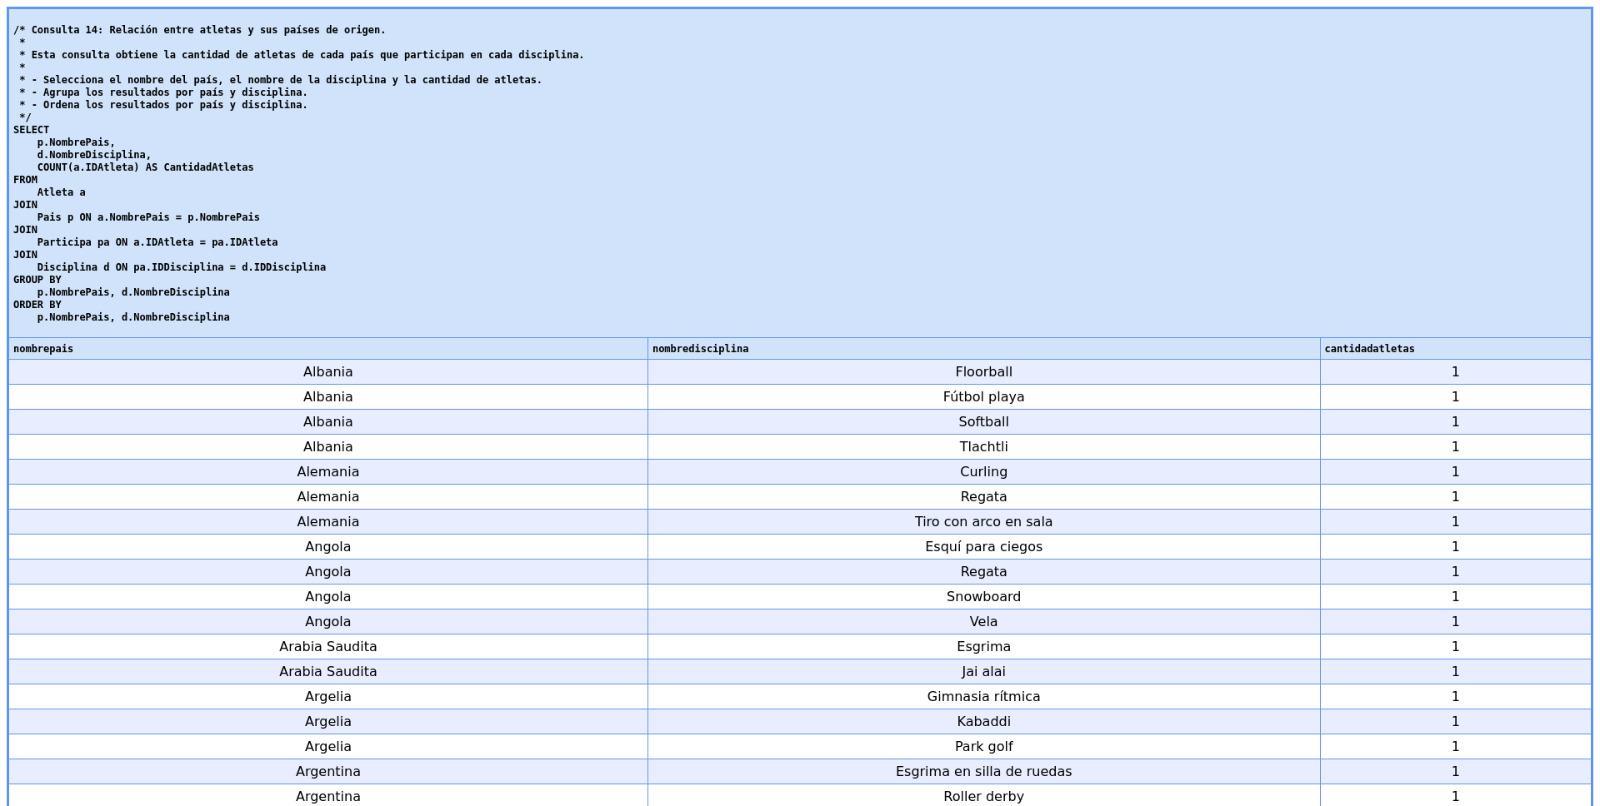
\includegraphics[width=16.5cm]{resources/Consulta14.jpeg} 
    
   Consulta 14. Relación entre atletas y sus países de origen.
\end{center}

\textbf{Propósito de la consulta}

El objetivo de esta consulta es obtener la cantidad de atletas de cada país que participan en cada disciplina. Esto permite analizar la representación de los países en diferentes disciplinas y evaluar la diversidad en las competencias deportivas.

\textbf{Desglose de la consulta}

\begin{itemize}
   \item \textbf{Selección de columnas (\texttt{SELECT})}:
   \begin{itemize}
       \item \texttt{p.NombrePais}: Nombre del país de origen de los atletas.
       \item \texttt{d.NombreDisciplina}: Nombre de la disciplina deportiva.
       \item \texttt{COUNT(a.IDAtleta)}: Calcula la cantidad de atletas por país en cada disciplina, generando la columna \texttt{CantidadAtletas}.
   \end{itemize}

   \item \textbf{Tablas involucradas (\texttt{FROM} y \texttt{JOIN})}:
   \begin{itemize}
       \item \texttt{Atleta (a)}: Contiene información sobre los atletas.
       \item \texttt{Pais (p)}: Contiene información sobre los países de origen.
       \item \texttt{Participa (pa)}: Relaciona a los atletas con las disciplinas en las que participan.
       \item \texttt{Disciplina (d)}: Contiene información sobre las disciplinas deportivas.
       \item Se realizan los siguientes \texttt{JOINs}:
       \begin{itemize}
           \item \texttt{Atleta} con \texttt{Pais} usando \texttt{a.NombrePais = p.NombrePais}, para asociar a cada atleta con su país de origen.
           \item \texttt{Atleta} con \texttt{Participa} usando \texttt{a.IDAtleta = pa.IDAtleta}, para identificar las disciplinas en las que participa cada atleta.
           \item \texttt{Participa} con \texttt{Disciplina} usando \texttt{pa.IDDisciplina = d.IDDisciplina}, para relacionar cada participación con una disciplina específica.
       \end{itemize}
   \end{itemize}

   \item \textbf{Agrupación de resultados (\texttt{GROUP BY})}:
   \begin{itemize}
       \item Los resultados se agrupan por \texttt{p.NombrePais} y \texttt{d.NombreDisciplina}, para calcular la cantidad de atletas por país en cada disciplina.
   \end{itemize}

   \item \textbf{Ordenamiento de resultados (\texttt{ORDER BY})}:
   \begin{itemize}
       \item Los resultados se ordenan primero por \texttt{p.NombrePais} (nombre del país) y luego por \texttt{d.NombreDisciplina} (nombre de la disciplina), facilitando la lectura y análisis.
   \end{itemize}
\end{itemize}

\textbf{Análisis detallado}

\begin{enumerate}
   \item \textbf{Relación entre tablas:}
   \begin{itemize}
       \item La consulta establece relaciones entre las tablas \texttt{Atleta}, \texttt{Pais}, \texttt{Participa} y \texttt{Disciplina}, conectando a cada atleta con su país y las disciplinas en las que participa.
   \end{itemize}
   
   \item \textbf{Cálculo de atletas:}
   \begin{itemize}
       \item La función agregada \texttt{COUNT(a.IDAtleta)} cuenta el número de atletas de un país que participan en cada disciplina.
   \end{itemize}
   
   \item \textbf{Agrupación:}
   \begin{itemize}
       \item El \texttt{GROUP BY} asegura que los datos estén organizados de manera que cada combinación de país y disciplina tenga su correspondiente conteo.
   \end{itemize}
   
   \item \textbf{Ordenamiento:}
   \begin{itemize}
       \item El orden jerárquico por país y disciplina facilita la interpretación, permitiendo identificar rápidamente la representación por país en cada deporte.
   \end{itemize}
\end{enumerate}

\textbf{Consideraciones}

\begin{itemize}
   \item \textbf{Atletas sin participación:}
   \begin{itemize}
       \item Si un atleta no está asociado a una disciplina, no aparecerá en los resultados.
   \end{itemize}
   \item \textbf{Empates en cantidad de atletas:}
   \begin{itemize}
       \item Si dos países tienen la misma cantidad de atletas en una disciplina, el orden entre ellos no está definido. Se podría agregar un criterio adicional en el \texttt{ORDER BY}, como el nombre del país o de la disciplina.
   \end{itemize}
\end{itemize}

\textbf{Utilidad de la consulta}

Esta consulta es útil para:
\begin{itemize}
    \item Analizar la diversidad de participación en cada disciplina y verificar la representación equitativa de diferentes países.
    \item Identificar posibles tendencias en la participación de atletas de determinados países en disciplinas específicas.
    \item Planificar estrategias de inclusión y promoción para fomentar la participación de países con poca representación.
    \item Facilitar reportes y estadísticas sobre la participación internacional en competencias deportivas.
\end{itemize}
